% Chapter Template

\chapter{Double Quantum Dot} % Main chapter title

\label{sec:DQD} % Change X to a consecutive number; for referencing this chapter elsewhere, use \ref{ChapterX}

%----------------------------------------------------------------------------------------
%	SECTION 1
%----------------------------------------------------------------------------------------

In this section we will focus on the study of a GaAs linear double quantum dot (DQD) array populated with two heavy holes (HH). 

\section{Hamiltonian and eigenstates}
The Hamiltonian of our model is described by Eq.~(\ref{eq:total_Hamiltonian}) which, by explicitly writing down all the terms, corresponds to
\begin{equation}
	\begin{split}
	\hat{\mathcal{H}}_{\text{DQD}}=&\sum_{i}\varepsilon_i\hat{n}_i+\sum_{i}U_i\hat{n}_{i\uparrow}\hat{n}_{i\downarrow}+\frac{1}{2}E_Z\sum_i(\hat{n}_{i\uparrow}-\hat{n}_{i\downarrow})\\
	&-t_N\sum_{i\neq j}\sum_{\sigma}\left(\hat{c}_{i\sigma}^\dagger c_{j\sigma}+\text{H.c.}\right)-t_F\sum_{i\neq j}\sum_{\sigma\neq \sigma'}\left(e^{i\theta_{ij}}\hat{c}_{i\sigma}^\dagger\hat{c}_{j\sigma'}+\text{H.c.}\right)\; ,
	\end{split}
\end{equation}
where we have defined the Zeeman splitting energy as $E_Z\equiv g^*\mu_B B$ with $g^*=1.45$ \cite{Bogan2017} for holes in GaAs under a perpendicular magnetic field. Like electrons, holes statistic are also given by the Fermi-Dirac distribution function, so if we want to obtain a matrix representation of the Hamiltonian we must use the fermionic anti-commutation property
\begin{equation}
\left\{\hat{c}_{i\sigma},\hat{c}_{j\sigma'}\right\}=\delta_{ij}\delta_{\sigma\sigma'}\; .
\end{equation}
With this property we can compute the matrix elements as
\begin{equation}
	\begin{split}
	\bra{\uparrow,\uparrow}\hat{\mathcal{H}}_{\text{DQD}}\ket{\uparrow,\uparrow}=\varepsilon_L+\varepsilon_R+E_Z\; ,
	\end{split}
\end{equation}
and for an off-diagonal element
\begin{equation}
	\begin{split}
	\bra{\uparrow,\uparrow}\hat{\mathcal{H}}_{\text{DQD}}\ket{0,\uparrow\downarrow}&=-t_Fe^{i\phi_{12}}\bra{\uparrow,\uparrow}\hat{c}_{L\uparrow}^\dagger\hat{c}_{R\downarrow}\ket{0,\uparrow\downarrow}\\
	&=-t_Fe^{i\theta_{12}}\bra{0,0}\hat{c}_{R\uparrow}\hat{c}_{L\uparrow}\hat{c}_{L\uparrow}^\dagger \hat{c}_{R\downarrow}\hat{c}_{R\uparrow}^\dagger\hat{c}_{R\downarrow}^\dagger\ket{0,0}\\
	&=-t_Fe^{i\theta_{12}}\bra{0,0}\hat{c}_{R\uparrow}\hat{c}_{R\downarrow}\hat{c}_{R\uparrow}^\dagger \hat{c}_{R\downarrow}^\dagger\ket{0,0}\\
	&=t_Fe^{i\theta_{12}}\bra{0,0}\hat{c}_{R\downarrow} \hat{c}_{R\downarrow}^\dagger\ket{0,0}\\
	&=t_Fe^{i\theta_{12}} \; .
	\end{split}
\end{equation}
With this we can write the Hamiltonian in the atomic basis as
\begin{equation}
	\hat{\mathcal{H}}_{\text{DQD}}=\bordermatrix{~ & \ket{\uparrow,\uparrow} & \ket{\uparrow,\downarrow} & \ket{\downarrow,\uparrow} & \ket{\downarrow,\downarrow} & \ket{\uparrow\downarrow,0} & \ket{0,\uparrow\downarrow}\cr
		~ & \varepsilon_L+\varepsilon_R+E_Z & 0 & 0 & 0 & -t_Fe^{i\theta_{12}} & t_Fe^{i\theta_{12}} \cr
		~ & 0 & \varepsilon_L+\varepsilon_R & 0 & 0 & -t_N & -t_N\cr
		~ & 0 & 0 & \varepsilon_L+\varepsilon_R & 0 & t_N & t_N\cr
		~ & 0 & 0 & 0 & \varepsilon_L+\varepsilon_R -E_Z & t_Fe^{i\theta_{12}} & -t_Fe^{i\theta_{12}}\cr
		~ & -t_Fe^{-i\theta_{12}} & -t_N & t_N & t_Fe^{-i\theta_{12}} &  2\varepsilon_L+U_L & 0 \cr
		~ & t_Fe^{-i\theta_{12}} & -t_N & t_N & -t_Fe^{-i\theta_{12}} &  0 & 2\varepsilon_R+U_R \cr}\; .
\end{equation}
In the experimental devices is typical to tune the intradot Coulomb interaction to be much greater in one dot than in the other one $U_L\gg U_R=U$ so we will work with the Hilbert subspace in which $\ket{\uparrow\downarrow,0}$ is not included. In this kind of systems the atomic basis in not the typical choice, so we change to the molecular basis Eq.~(\ref{eq:molecular_basis}) and the Hamiltonian reads as
\begin{equation}
\hat{\mathcal{H}}_{\text{DQD}}=\bordermatrix{~ & \ket{T_+(1,1)} & \ket{T_0(1,1)} & \ket{T_-(1,1)} & \ket{S(0,2)} & \ket{S(1,1)}\cr
	~ & E_Z & 0 & 0 & t_Fe^{i\theta_{12}} & 0 \cr
	~ & 0 & 0 & 0 & 0 & 0\cr
	~ & 0 & 0 & -E_Z & -t_Fe^{i\theta_{12}} & 0 \cr
	~ & t_Fe^{-i\theta_{12}} & 0 & -t_Fe^{-i\theta_{12}} & 2\varepsilon_R+U & -\sqrt{2}t_N \cr
	~ & 0 & 0 & 0 & -\sqrt{2}t_N &  \varepsilon_L+\varepsilon_R  \cr}\; .
\label{eq:Hamiltonain_DQD_2HH_Full}
\end{equation}
Here we can see that the triplet state $\ket{T_0(1,1)}$ is not coupled to any state it will not be considered for the rest of the chapter. Furthermore, if the magnetic field is high enough we can also neglect one more triple state $\ket{T_+(1,1)}$. The detuning between dots is defined as $\varepsilon\equiv \varepsilon_R-\varepsilon_L$, in order to decrease the number of free parameters we fix $\varepsilon_L=-\varepsilon_R$, so the final effective Hamiltonian is
\begin{equation}
\hat{\mathcal{H}}_{\text{DQD}}^{\text{eff.}}=\bordermatrix{~ & \ket{T_-(1,1)} & \ket{S(0,2)} & \ket{S(1,1)}\cr
	~ & -E_Z & -t_Fe^{-i\theta_{12}} & 0 \cr
	~ & -t_Fe^{-i\theta_{12}} & \varepsilon +U & -\sqrt{2}t_N \cr
	~ & 0 & -\sqrt{2}t_N &  0  \cr}\; .
\label{eq:effective_Hamiltonian_DQD}
\end{equation}
The characteristic polynomial of this matrix corresponds to
\begin{equation}
	\abs{\hat{\mathcal{H}}_{\text{DQD}}^{\text{eff.}}-\lambda\mathds{1}}=(\varepsilon+U-\lambda)\lambda^2+\lambda\left[(\varepsilon+U-\lambda)E_Z+t_F^2\right]+2(\lambda+E_Z)t_N^2=0\; ,
\end{equation}
which has no dependence on the complex phase se we set $\theta_{12}=0$ for the rest of the work. Let's denote with $\ket{\phi_i}$ the instant eigenstates and $E_i$ the energies of the system whose spectrum can be found in Fig.~\ref{fig:eigenenergies_DQD_2HH}. This energy spectrum corresponds to the Hamiltonian given in Eq.~(\ref{eq:Hamiltonain_DQD_2HH_Full}), before neglecting the two triplet states commented above. In order to fix a notation we will denote with $\ket{\phi_0}$ the lowest energy state (blue), $\ket{\phi_1}$ the first excited state (red) and so on up to $\ket{\phi_4}$ for the most energetic instant state. The results coincide with those obtained by other experimental groups \cite{SachrajdaUnpublished}.
\begin{figure}[!htbp]
	\centering
	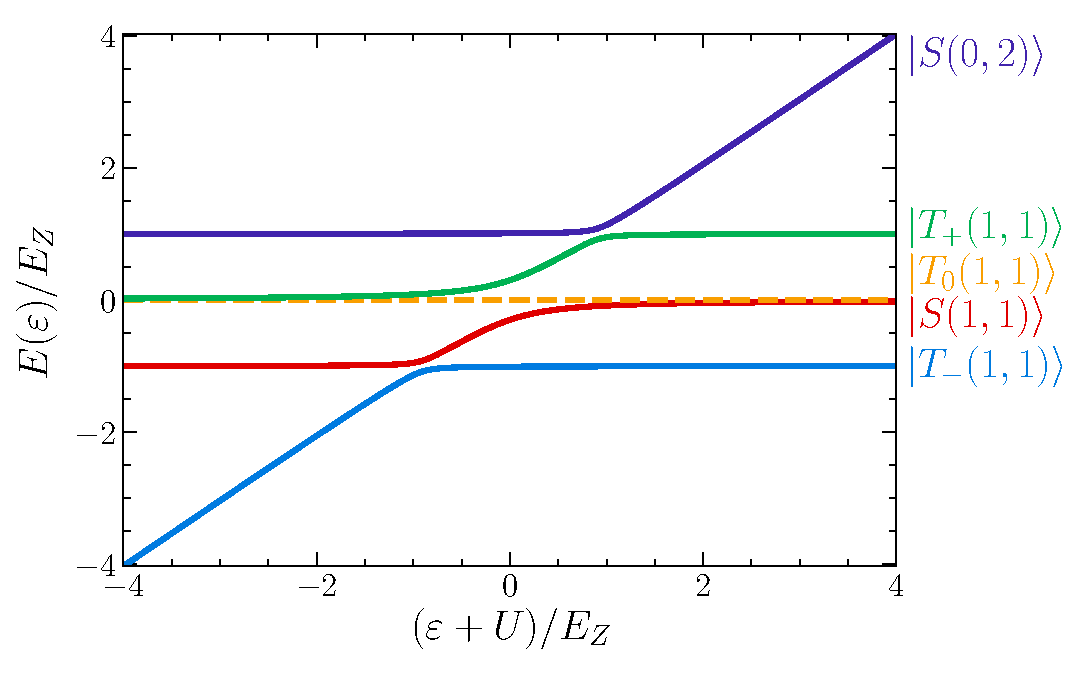
\includegraphics[width=0.8\linewidth]{eigenenergies_DQD_2HH.eps}
	\caption{Energy spectrum for a GaAs DQD populated with two HH. The parameters used are $E_Z=1.17\; \mu$eV, $U=2$ meV, $t_N=0.25\; \mu$eV and $t_F=0.1\; \mu$eV. At the right of each instant state we have specified the corresponding element in the molecular basis in the high detuning limit.}
	\label{fig:eigenenergies_DQD_2HH}
\end{figure}

Our aim in this chapter is to find a protocol with which the system can be transferred from the triplet state $\ket{T_-(1,1)}$ to the single occupation singlet state $\ket{S(1,1)}$. This transition can be obtained by varying the detuning of the QD's from $(\varepsilon+U)\ll-E_Z$ to $(\varepsilon+U)\gg E_Z$. In our model we have not included any term that allows the spin flip of a particle without tunneling to other dot, so the only possible path would be
\begin{equation}
	\ket{\downarrow,\downarrow}\rightarrow\ket{0,\uparrow\downarrow}\rightarrow\frac{1}{\sqrt{2}}(\ket{\uparrow,\downarrow}-\ket{\downarrow,\uparrow})\; .
\end{equation}
This can be done by following adiabatic state $\phi_1$, but with the inconvenience that the charge change it's location, producing the undesired charge noise. We can mitigate with effect if we can find an instant eigenstate which has no weight if the double occupation state, also known as dark state. The adiabatic state can be written generically as
\begin{equation}
	\ket{\phi_1}=a_1\ket{S(1,1)}+a_2\ket{S(0,2)}+a_3\ket{T_-(1,1)}\; .
	\label{eq:adiabatic_state}
\end{equation}
The eigenstates has not a nice analytical solution, so we have opted to find the dark state by solving numerically the instant eigenstates of the system. There are many different variables in the system so we fix the Coulomb interaction $U$ and the Zeeman splitting $E_Z$, and change the detuning $\varepsilon$ and the spin-conserving tunneling rate $t_N$. The spin-flip tunneling rate can be experimentally tune independently of $t_N$, in this chapter we will restrict ourselves to a constant value of $t_F=0.1\; \mu$eV, what is in line with some experimental data \cite{Bogan2018}. The numerical results for the the population of the double occupation singlet state ($\abs{a_2}^2$ in Eq.~(\ref{eq:adiabatic_state})) in terms of the detuning and the tunneling rate is shown in Fig.~\ref{fig:occupation_middle_state}. As we have said before, the desired transference is only achievable if the detuning goes from $(\varepsilon+U)\ll -E_Z$ to $(\varepsilon+U)\gg 0$. This means that if we want to suppress the population of the double occupation singlet state during the transference we must set a high spin-conserving tunneling rate $t_N\sim 5\mu$eV.
\begin{figure}[!htb]
	\centering
	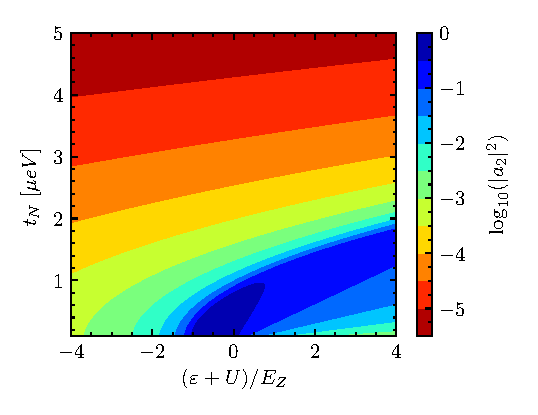
\includegraphics[width=0.6\linewidth]{occupation_middle_state.eps}
	\caption{Population of the double occupation singlet state $\ket{S(0,2)}$ in the first excited instant state $\ket{\phi_1}$, where we have defined $\abs{a_1}^2\equiv \abs{\braket{S(0,2)}{\phi_1}}^2$. All the other parameters are the same than in Fig.~\ref{fig:eigenenergies_DQD_2HH}.}
	\label{fig:occupation_middle_state}
\end{figure}


Other aspect that is worth to discuss is the initial and final values for the detuning. The ideal scenario would be that the adiabatic state corresponds to the target states at the beginning and the end of the protocol, i.e. $\ket{\phi_1(t=0)}=\ket{T_-(1,1)}$ and $\ket{\phi_1(t=t_f)}=\ket{S(1,1)}$, but this is only possible in the limit $\varepsilon:[-\infty,+\infty]$, what is impossible to achieve experimentally. The values for $\abs{a_1}^2$ and $\abs{a_3}^2$ in term of the detuning and the tunneling $t_N$ is shown in Fig.~\ref{fig:limits_FAQUAD}. Note that what is represented is the not exactly the population but how close it's to the unity in logarithmic scale. Here we can see that when we increase the value for the tunneling rate in order not to populate the double occupation doublet state, and fixed the values $\abs{a_3(t=0)}^2$ and $\abs{a_1(t=t_f)}^2$, the total range for the detuning becomes wider which results in a higher energy expenditure. We must find a equilibrium between high fidelities and a reasonable limits for the detuning, this is why for the rest fo the chapter set the initial and final detuning values such that $\abs{a_3(t=0)}^2=0.9999$ and $\abs{a_1(t=t_f)}^2=0.9999$. If better fidelity is needed we can always  increase the range used for detuning.\\
\begin{figure}[!htb]
	\centering
	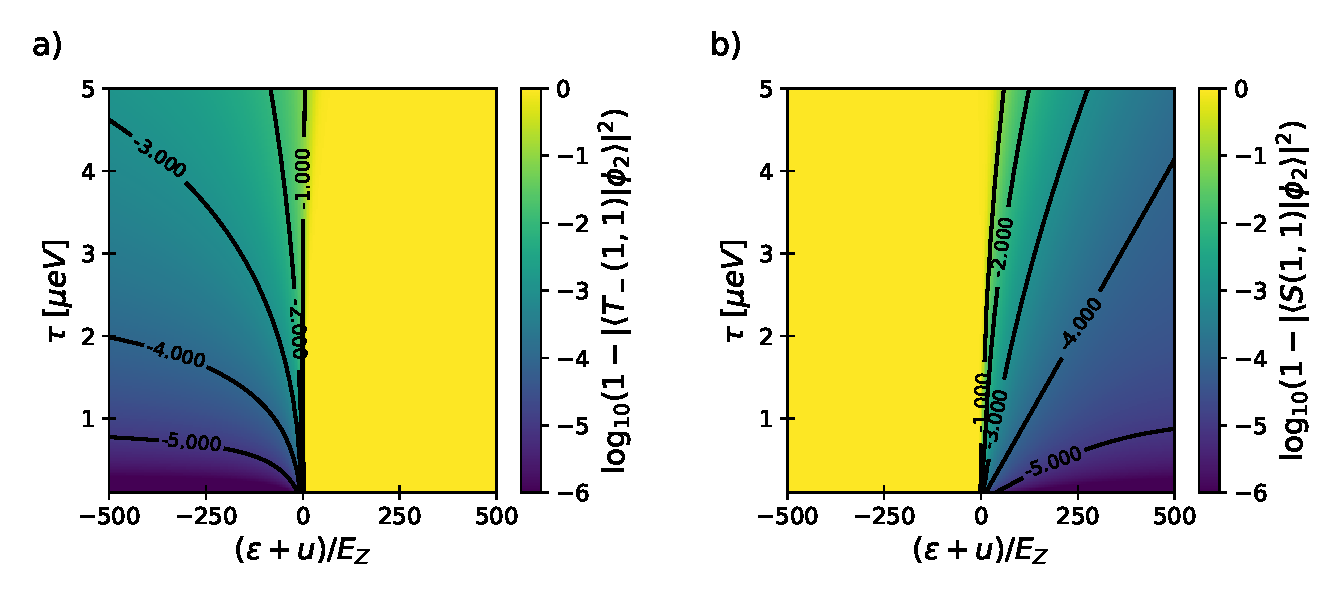
\includegraphics[width=\linewidth]{limits_FAQUAD.eps}
	\caption{Population of a) the triplet state and b) the single occupation singlet state in terms of the detuning and the spin-conserving tunneling rate. All the other parameters are the same than in Fig.~\ref{fig:eigenenergies_DQD_2HH}.}
	\label{fig:limits_FAQUAD}
\end{figure}

Now we must choose what STA scheme we will use in the system. As we have mentioned before it's not easy to obtain an analytical expression for the three instant eigenvectors so we rule out the use of CD. We are dealing with a three level system what means that the eigenstates can be conveniently obtained numerically and considering that with these we obtain all the information in the system we decided to go for the use of FAQUAD.
\section{FAQUAD Results}
The parameters that we will use are a Zeeman splitting of $E_Z=1.17\: \mu$eV, what correspond to a magnetic field $B\sim 15$ mT, an intradot Coulomb interaction of $U= 2$ meV, and a spin-flip tunnelling rate of $t_F=0.1\; \mu$ eV. Let's start choosing a moderate value for the spin-conserving tunnelling rate of $t_N=0.25\; \mu$eV with which the double occupation singlet will be occupied. This will serve us as a first test to verify that FAQUAD protocol achieves the target state with fidelities close to the unit. In the following we will use the definition for the adimensional detuning $\tilde{\varepsilon}\equiv (\varepsilon+U)/E_Z$ to shorten the notation in the text, although the original notation will be retained in the figures for clarity. With the above values for the parameters of the system we can compute numerically the initial and final detuning to obtain $\abs{a_1(t=0)}^2=\abs{a_3(t=t_f)}^2=0.9999$ obtaining $\tilde{\varepsilon}(t=0)=-10.08$ and $\tilde{\varepsilon}(t=t_f)=30.15$. Together with the eigenstates and eigenenergies that we can obtain numerically we can introduce them in Eq.~(\ref{eq:c_tilde_deff}) identifying $\lambda(t)=\varepsilon(t)$ and the initial state as $\ket{\phi_1}$, by which we want to perform the adiabatic transfer. With this we obtain a value for the rescaled adiabatic parameter $\tilde{c}=4.34$ ns, so if we want an adiabatic passage $c=\tilde{c}/t_f\ll 1$ we need times $t_f\sim 100$ ns. Now introducing this factor in Eq.~(\ref{eq:parameter_ODE_2}) we can solve by numerical integration the dependence of the detuning with the rescaled time $s\equiv t/t_f$, what is shown in Fig.~\ref{fig:FAQUAD_detuning_2QD_2HH} a). What is more interesting is how the rate of change, i.e the speed, of the detuning varies as we approach or move away from the avoided crossings. In Fig.~\ref{fig:FAQUAD_detuning_2QD_2HH} b) we can see that near $\tilde{\varepsilon}=-1$ and $\tilde{\varepsilon}=0$, where avoided crossings are located, the detuning slows down to ensure an adiabatic passage. Nevertheless, as the energies are away from each other the detuning speeds up to get the shortest possible final times. The obtained shape is smooth so the detuning implementation in a real life experiment is feasible.
\begin{figure}[!htbp]
	\centering
	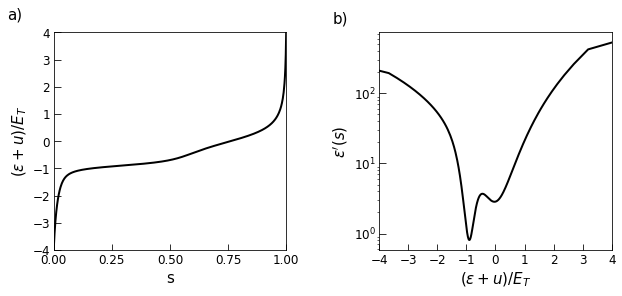
\includegraphics[width=0.9\linewidth]{FAQUAD_detuning_2QD_2HH.pdf}
	\caption{a) Dependence of the detuning in terms of the rescaled time $s=t/t_f$ obtained by solving numerically the FAQUAD protocol. b) Derivative of the detuning in terms of the detuning itself. The spin-conserving tunnelling used is $t_N=0.25\; \mu$eV, all the other parameters are the same than in Fig.~\ref{fig:eigenenergies_DQD_2HH}.}
	\label{fig:FAQUAD_detuning_2QD_2HH}
\end{figure}

Let's define the fidelity of the protocol as
\begin{equation}
	\mathcal{F}(t_f)\equiv \abs{\braket{\phi_1(t_f)}{\Psi(t_f)}}^2\; ,
\end{equation}
where $\ket{\Psi(t)}$ represent the solution of the time dependent Schrödinger equation. We solve the density matrix dynamics equation for several final times, what is shown in Fig.~\ref{fig:FAQUAD_2QD_Results}. As we have predicted by adiabatic perturbation theory Eq.~(\ref{eq:FAQUAD_fidelity}), the fidelity has a wavy behaviour governed by two frequencies. As the final time grows the fidelity is stabilized at a value close to unity. The first peak is reached at $t_f=27.34$ ns, obtaining a fidelity of $\mathcal{F}=0.98$. The evolution of the states at this final time can be seen in Fig.~\ref{fig:states_evolution_1}. The target state $\ket{S(1,1)}$ is reached at the end of the passage, but in the meantime the double occupation singlet state has a population considerably high. The maximum population of this state for the other peaks in the fidelity are no lower, reaching values of $\abs{\braket{S(0,2)}{\Psi(t_f)}}^2\sim 0.8$.\\
\begin{figure}[!htb]
	\centering
	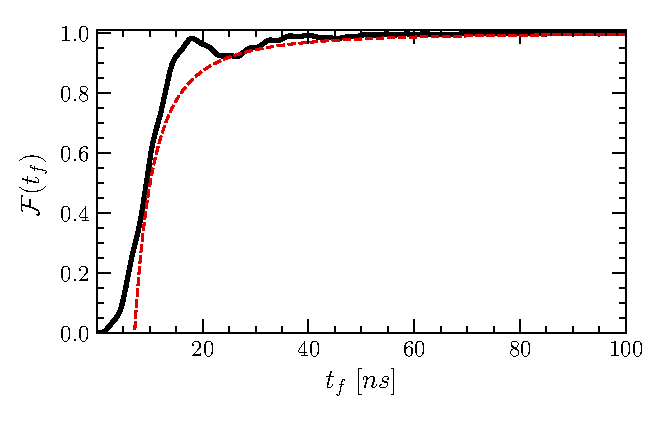
\includegraphics[width=0.7\linewidth]{FAQUAD_2QD_Results.eps}
	\caption{Fidelity in term of the final time. The spin-conserving tunnelling used is $t_N=0.25\; \mu$eV, all the other parameters are the same than in Fig.~\ref{fig:eigenenergies_DQD_2HH}.}
	\label{fig:FAQUAD_2QD_Results}
\end{figure}
\begin{figure}[!htb]
	\centering
	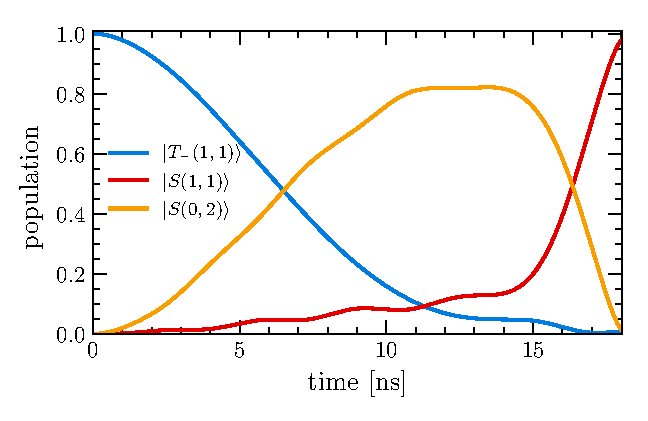
\includegraphics[width=0.7\linewidth]{states_evolution_1.eps}
	\caption{Population for the different states during the protocol with a final time of $t_f=27.34$ ns. The fidelity at this time is $\mathcal{F}=0.98$. The spin-conserving tunnelling used is $t_N=0.25\; \mu$eV, all the other parameters are the same than in Fig.~\ref{fig:eigenenergies_DQD_2HH}.}
	\label{fig:states_evolution_1}
\end{figure}

In order to decrease the population of $\ket{S(0,2)}$ we must use higher values for the spin-conserving tunneling rates as we have seen in Fig.~\ref{fig:occupation_middle_state}, let's use for instance $t_N=5\; \mu$eV. In order to keep the initial and final populations in the adiabatic state of $\abs{a_1(t=0)}^2=0.9999$ and $\abs{a_3(t=t_f)}^2=0.9999$ we must increase the range for the detuning. With the new tunneling rates we obtain that $\tilde{\varepsilon}(0)=-18.18$ and $\tilde{\varepsilon}(t_f)=619.21$ for the initial and final time respectively. With this parameters we obtain $\tilde{c}=21.42$ ns, so the final times must be greater than those previously used with a smaller tunneling rate. In Fig.~\ref{fig:FAQUAD_detuning_2QD_2HH_2} we have shown the detuning and its derivative. The qualitative behaviour is very similar to that obtained previously in Fig.~\ref{fig:FAQUAD_detuning_2QD_2HH}, with the difference that now the two avoided crossings are so close to each other that we only appreciate one minimum in the derivative.
\begin{figure}[!htb]
	\centering
	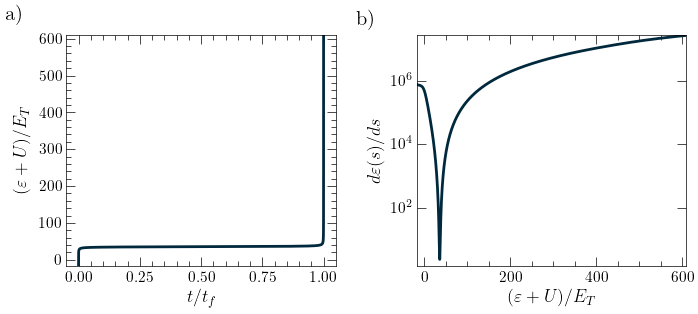
\includegraphics[width=0.92\linewidth]{FAQUAD_detuning_2QD_2HH_2.pdf}
	\caption{a) Dependence of the detuning in terms of the rescaled time $s=t/t_f$ obtained by solving numerically the FAQUAD protocol. b) Derivative of the detuning in terms of the detuning itself. The spin-conserving tunnelling used is $t_N=5\; \mu$eV, all the other parameters are the same than in Fig.~\ref{fig:eigenenergies_DQD_2HH}.}
	\label{fig:FAQUAD_detuning_2QD_2HH_2}
\end{figure}

The fidelity for $t_N=5 \; \mu$eV is shown in Fig.~\ref{fig:FAQUAD_2QD_Results_2}. As we have predicted the total time needed for reaching the first peak, $t_f=112.88$ ns, is much larger than before. However, the fidelity has improved reaching a value of $\mathcal{F}=0.99998$ at the first peak. Using Eq.~(\ref{eq:FAQUAD_frecuencies}) we predict two periods of $T_1=120$ ns and $T_2=0.14$ ns. The first one can be easily seen in the results for the fidelity, but $T_2$ is so small that cannot be seen with the naked eye. In order to visualize it, which corresponds to a frequency of $\nu_2=1/T_2\sim 7.14$ ns$^{-1}$, we can numerically compute the Fourier transform for the fidelity Fig.~\ref{fig:frecuency_spectrum}, obtaining a peak in a frequency close to the predicted one.
\begin{figure}[!htb]
	\centering
	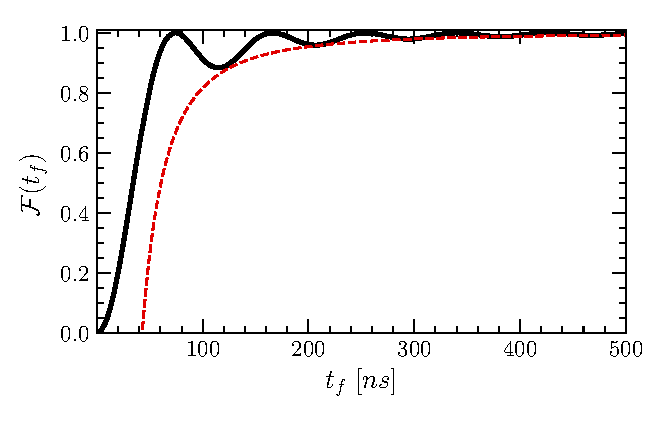
\includegraphics[width=0.7\linewidth]{FAQUAD_2QD_Results_2.eps}
	\caption{Fidelity in term of the final time. The spin-conserving tunnelling used is $t_N=5\; \mu$eV, all the other parameters are the same than in Fig.~\ref{fig:eigenenergies_DQD_2HH}.}
	\label{fig:FAQUAD_2QD_Results_2}
\end{figure}
\begin{figure}[!htb]
	\centering
	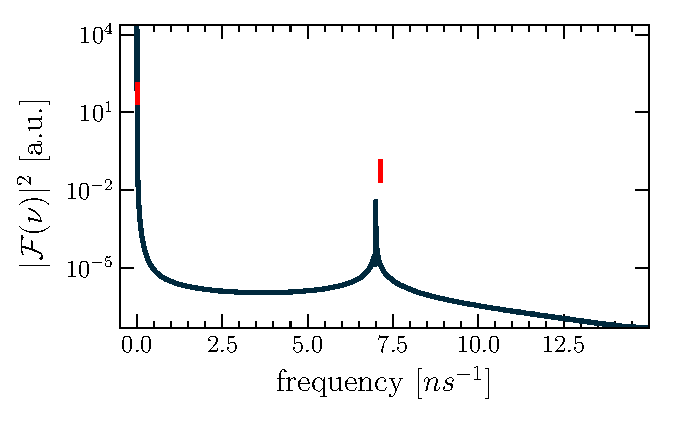
\includegraphics[width=0.7\linewidth]{frecuency_spectrum.eps}
	\caption{Fourier transform in arbitrary units for the fidelity shown in Fig.~\ref{fig:FAQUAD_2QD_Results_2}. The two red lines corresponds to the frequencies predicted at first order in adiabatic perturbation theory.}
	\label{fig:frecuency_spectrum}
\end{figure}

The purpose of increasing the spin-conserving tunneling rate was to mitigate the charge noise by decreasing the total population of the double occupation singlet state $\ket{S(0,2)}$. In Fig.~\ref{fig:states_evolution_2} we have plotted the evolution for the different states of the system for a total time corresponding to the first peak in the fidelity. We can seen that the population of $\ket{S(0,2)}$ has decreased with respect to a lower tunneling rate, obtaining a maximum value of $2.5\%$ during the transference. This value remains constant for all other peaks in fidelity.
\begin{figure}[!htb]
	\centering
	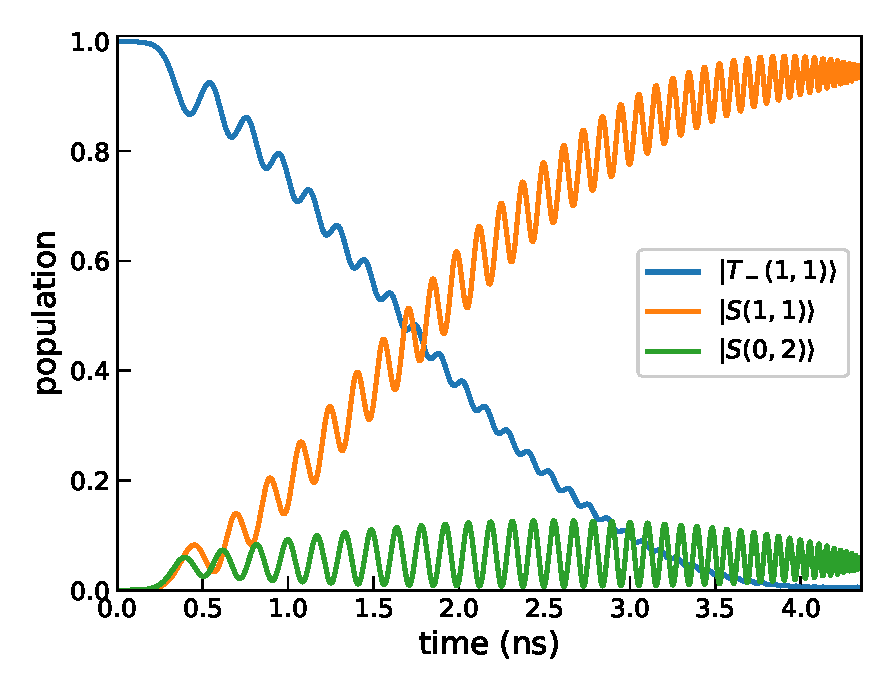
\includegraphics[width=0.7\linewidth]{states_evolution_2.eps}
	\caption{Population for the different states during the protocol with a final time of $t_f=112.88$ ns. The fidelity at this time is $\mathcal{F}=0.99998$. The spin-conserving tunnelling used is $t_N=5\; \mu$eV, all the other parameters are the same than in Fig.~\ref{fig:eigenenergies_DQD_2HH}.}
	\label{fig:states_evolution_2}
\end{figure}

All the results that we have given so far was obtained by using the effective Hamiltonian shown ins Eq.~(\ref{eq:effective_Hamiltonian_DQD}). We can include the triplet state $\ket{T_+(1,1)}$ and repeat the FAQUAD protocol now with three terms in the summatory of Eq.~(\ref{eq:parameter_ODE_2}). Computing the fidelity obtained in terms of the total time we get that the first peak is reached at $t_f=105.6$ ns, a slightly quicker than when working with the effective Hamiltonian. The fidelity in this peak corresponds to $\mathcal{F}=0.99990$, way to close to the previously value. The time evolution of the system (not shown here) is also quite similar to when we only deal with a three level system, so the use of the effective Hamiltonian is justified. In order to save computation time we will stick to this effective model for the rest of the chapter.


\section{One qubit gate}
Now that we have been able to achieve a negligible population in the double occupation singlet state, we are dealing with a two level system, so the map with a qubit is natural. Let's call $\ket{0}\equiv\ket{T_-(1,1)}$ and $\ket{1}\equiv \ket{S(1,1)}$ the computational basis. In order to represent the two degrees of freedom present in a qubit it's usual to work with the Bloch sphere, in which each pole represent a element of the computation basis. The superposition of $\ket{0}$ and $\ket{1}$ is given by the polar angle $0\leq \theta\leq \pi$, and the azimuthal angle $0\leq\phi<2\pi$. A general wave function can be written as
\begin{equation}
	\ket{\Psi}=r\cos(\theta/2)\ket{0}+e^{i\phi}\sin(\theta/2)\ket{1}\; ,
\end{equation}
where we have introduced the radius $0<r\leq 1$ to take into account a possible leakage of the computation basis. In Fig.~\ref{fig:Bloch_sphere_combined} a) we have plotted the trajectory in the Bloch sphere followed by the system as the total time for the FAQUAD protocol varies.
\begin{figure}[!htb]
	\centering
	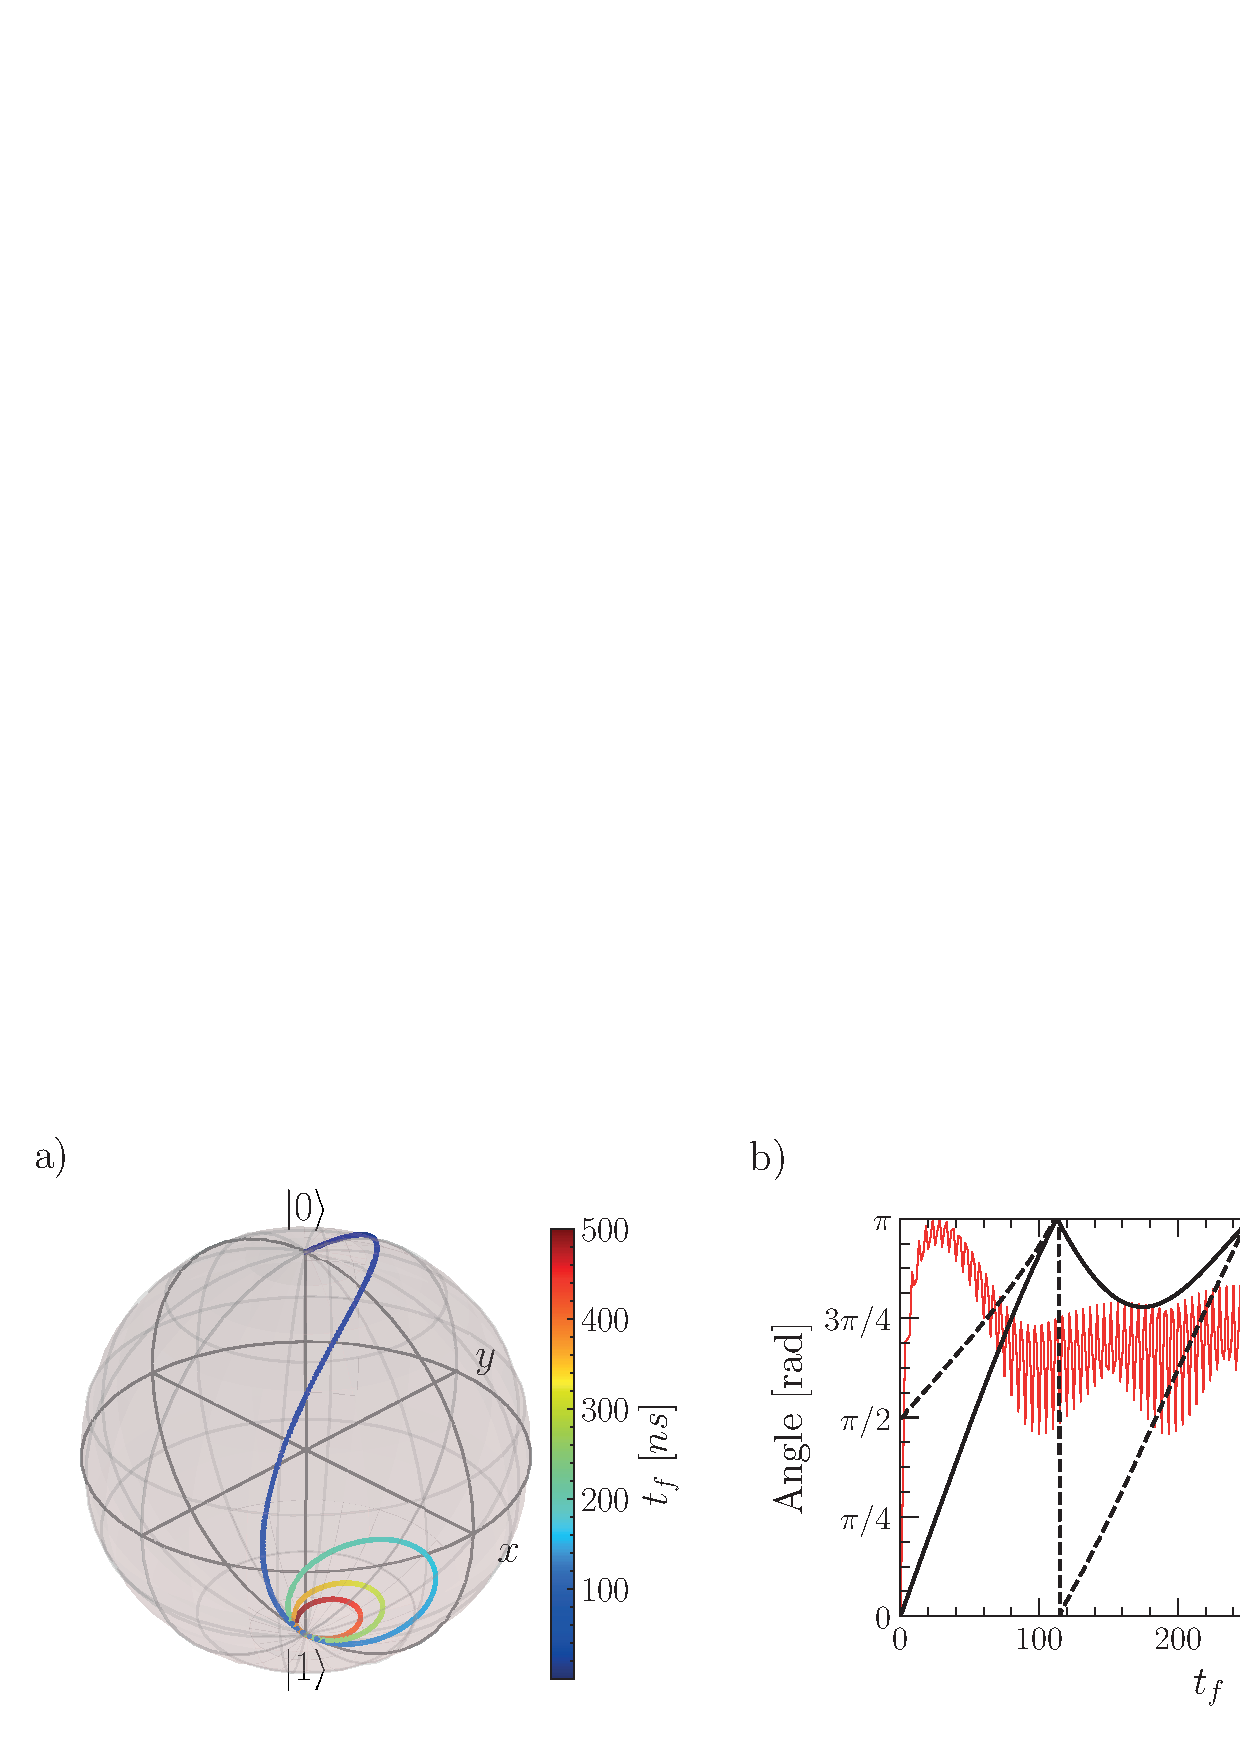
\includegraphics[width=\linewidth]{Bloch_sphere_combined.pdf}
	\caption{a) Trajectory for the system in the Bloch sphere in terms of the final time. We have identified $\ket{0}\equiv\ket{T_-(1,1)}$ and $\ket{1}\equiv \ket{S(1,1)}$. b) Evolution for the polar angle $\theta$ (solid black), the azimuthal angle (dashed black) $\phi$ and the radius (solid red). The spin-conserving tunnelling used is $t_N=5\; \mu$eV, all the other parameters are the same than in Fig.~\ref{fig:eigenenergies_DQD_2HH}.}
	\label{fig:Bloch_sphere_combined}
\end{figure}

We are able to rotate a state from the north pole $\ket{0}$ to the south pole $\ket{1}$ including all intermediate values of the polar angle. This angle can be modified vie the final time $t_f$, Fig.~\ref{fig:Bloch_sphere_combined}, so we have total control over this parameter. To be able to reach any point on the sphere of Bloch we must be able to rotate a state on the z axis, what can be done by letting the system evolve with a time independent Hamiltonian, the acquired phase can be written as
\begin{equation}
	\phi_a(t)=-\frac{1}{\hbar}\int_0^t dt'[E_{S(1,1)}-E_{T_-(1,1)}]=-\frac{E_Z}{\hbar}t\; .
\end{equation}
The maximum acquired phase that we must need is $\phi_a=2\pi$, which can be achieved in a time $t=2\pi\hbar/E_Z$. Using a value of $E_Z=1.17\; \mu$eV this corresponds to a time of $t=3.5$ ns. This rotation can be speed up or slow down by decreasing or increasing the magnetic field respectively. Then we have total control over $\theta$ and $\phi$, so we can prepare our qubit in an arbitrary state in at most $120$ ns. This constitute a general one qubit quantum gate. The dependences of $\theta$ and $\phi$ with the total time $t_f$ has a really simple behaviour and can be fitted by a first or second order polynomial function, so it's easy to extract the time needed to achieved a certain value. Possible leaks outside the computer base are limited to $(1-r)^2=6.4\times10^{-3}\%$ at most, as shown in Fig.~\ref{fig:Bloch_sphere_combined} b) (red).
\section{Systematic and stochastic errors}


